\documentclass{article}
\usepackage[T1]{fontenc}
\usepackage{lmodern}
\usepackage{graphicx}
\usepackage{amsmath,amssymb}
\usepackage[a4paper,margin=2cm]{geometry}
\usepackage[absolute,overlay]{textpos}
\setlength{\TPHorizModule}{1mm}
\setlength{\TPVertModule}{1mm}
\usepackage[indonesian]{babel}
\usepackage{hyperref}
\setlength{\emergencystretch}{2em}
% unit: Halaman 30

\begin{document}

% === Halaman 30 (llm) ===

\vspace{137.21mm}

Istilah keilmuan serumpun terasa memberikan distorsi persepsi pada maksud sebenarnya. Persepsi yang segera terbentuk dengan istilah tesrebut adalah pertumbuhan dari akar-akar ilmu membentuk suatu rumpun, yang berarti bahwa nuansa historis organisasi/kelompok/unit yang mewadahinya.\\ \vspace{10mm} \begin{tabular}{ccc} Embedded message & Cover-image & Stego-image \end{tabular}

% deskripsi: Gambar cover-image yang menunjukkan sekumpulan paprika warna-warni.
% bbox normalisasi: [0.3340, 0.2120, 0.5880, 0.6740]
\begin{textblock*}{53.34mm}(70.14mm,62.96mm)
\noindent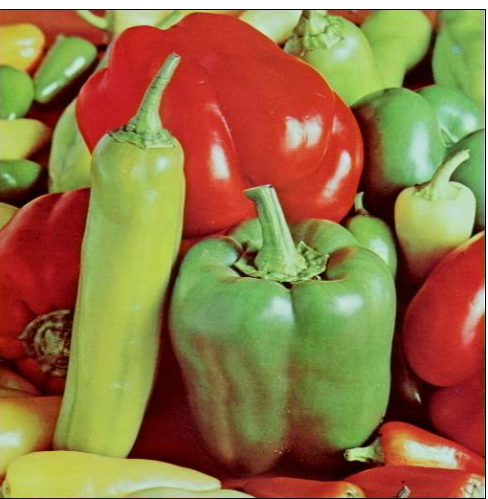
\includegraphics[width=53.34mm,height=137.21mm]{../../images/llm/page_030_img_01.png}%
\end{textblock*}

% deskripsi: Gambar stego-image yang terlihat identik dengan cover-image, digunakan untuk mengilustrasikan steganografi.
% bbox normalisasi: [0.6030, 0.2120, 0.8580, 0.6740]
\begin{textblock*}{53.55mm}(126.63mm,62.96mm)
\noindent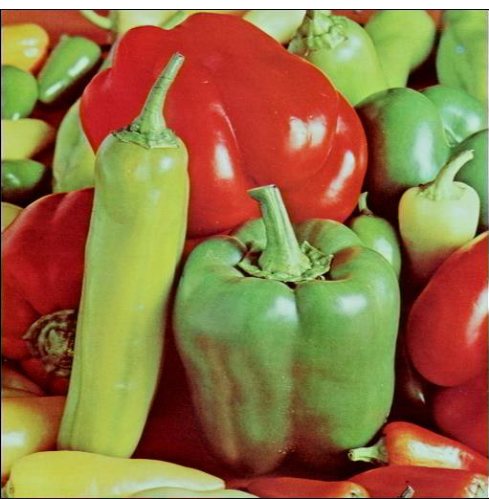
\includegraphics[width=53.55mm,height=137.21mm]{../../images/llm/page_030_img_02.png}%
\end{textblock*}

\end{document}
